\documentclass{beamer}
\title{Applications of Computer Vision}
\author{Ajit}
\date{\today}
\usepackage{color,graphicx,amssymb,multimedia,smartdiagram,tikz}
\usetheme{Warsaw}
\usepackage{media9}
\usepackage[utf8]{inputenc}
\usepackage{lmodern}
\usepackage{subfig}
\usepackage{wrapfig}
\usepackage{blindtext}
\usepackage[T1]{fontenc}
\usebackgroundtemplate%

\title{Computer Vision}
\author{\emph{Bhupender Yadav\\
		Prince Jangra\\
		Khubaib Raza\\
		Karan Yadav\\
		Ajit Yadav}
}
\institute{\emph{University OF Delhi}}
\begin{document}
	{
		\usebackgroundtemplate{%
			\tikz\node[opacity=0.9] {\includegraphics[height=\paperheight,width=\paperwidth]{front}};}
		\begin{frame}
		\titlepage
	\end{frame}
}
{
	\usebackgroundtemplate{%
		\tikz\node[opacity=0.5] {\includegraphics[height=\paperheight,width=\paperwidth]{grey}};}
	\begin{frame}{Acknowledgement}
	I will like to offer my great appreciation to all my group members.\\I would like to offer my special thanks to \textbf{LESLIE LAMPORT} for inventing such a great typesetting programme.\\ I would like to express my very great appreciation to \textbf{Mr.Nikhil Khanna} for his valuable and constructive suggestions during the planning and development of this research work.His willingness to give his time time so generously has been very much appreciated.\\
	My \textbf{SPECIAL THANKS} are extended to the staff of \textbf{"DEPARTMENT OF MATHEMATICS"}.
\end{frame}
{
	\usebackgroundtemplate{%
		\tikz\node[opacity=0.4] {\includegraphics[height=\paperheight,width=\paperwidth]{Wall1}};}
	
	\begin{frame}{Wall1}
	\frametitle{Overview}
	\begin{itemize}
		\item Introduction
		\item Histroy Of Computer Vision
		\item Applications
		\item Typical Task
		\item Scope of Computer Vision
		\item System Methods
		\item Reference
	\end{itemize}
\end{frame}
}

{
	\usebackgroundtemplate{%
		\tikz\node[opacity=0.5] {\includegraphics[height=\paperheight,width=\paperwidth]{butterfly}};}
	
	\begin{frame}
	
	\begin{abstract}
		The field of computer vision is devoted to discovering algorithms, data representations, and computer architectures that embody the principles underlying visual capabilities. This article describes how the field of computer (and robot) vision has evolved, particularly over the past 20 years, and introduces its central methodological paradigms.
	\end{abstract}
\end{frame}
}

{\pgfdeclareimage[height=\paperheight,width=\paperwidth]{myimage}{cv9}
\usebackgroundtemplate{\tikz\node[opacity=1] {\pgfuseimage{myimage}};}
\begin{frame}[t]
%\begin{block}

%\centering{\Huge{\textbf{\color{magenta}{Applications of}}}}

%\end{block}
\end{frame}
}

\begin{frame}

\centering{\Large{\textbf{Applications of Computer Vision}}}


\begin{block}
	
		Computer Vision, an Artifecial Intelligence(AI) technology that allows computers to understand \& label images, is now used in convenienc stores, driverless car testing, daily medical diagonistics \& in monitoring the health of crops and livestock.
	
	\vspace{.75cm}
	
	Computer Vision is a booming industry that is being applied to many of our every day products.We have seen that computers are proficient at recognizing images. Today, top technology companies such as \textbf{\color{cyan}{amazon}}, {\color{blue}{G}\color{red}{o}\color{yellow}{o}\color{blue}{g}\color{green}{l}\alert{e}},\textbf{\color{gray}{Microsoft}} \& \textbf{\color{blue}{facebook}} are investing billion of dollars(\$) in Computer Vision research and product development.
	
	\vspace{.75cm}
	
	From my research, I've found that many of those use cases of computer vision fall into the following clusters.
	
	\end{block}

\end{frame}


{\pgfdeclareimage[height=\paperheight,width=\paperwidth]{myimage}{Smart}
\usebackgroundtemplate{\tikz\node[opacity=.4] {\pgfuseimage{myimage}};}
\begin{frame}[t]{Applications}
\centering{\smartdiagramanimated[bubble diagram]{Computer\ Vision,
  Retail, Automotive, Sequrity, Healthcare, Robotics}}

\end{frame}
}
{\pgfdeclareimage[height=\paperheight,width=\paperwidth]{myimage}{az.jpeg}
\usebackgroundtemplate{\tikz\node[opacity=.4] {\pgfuseimage{myimage}};}
\begin{frame}[t]{\underline{(1).Retail}}
\setbeamercolor{block body}{use=structure,fg=black,bg=purple!40!white}

\begin{exampleblock}
	
	\color{cyan}{Some early applications of Computer Vision in retail come from e-commerce, but increasingly, it is being used in physical retail stores to perfect shelf merchandising, enhance operational efficiencies and create a frictionless experience for shoppers.}
	
\end{exampleblock}

\begin{columns}[t]
\pause
	\begin{column}{5cm}
		
		\centering{\textbf{\alert{Amazon Go}}}\\
\small{Amazon recently opened to the public the Amazon Go stores where shoppers need not wait in lines at the checkout center to pay for their purchases.\\}
			%
		\href{run:Amazon Go.mp4}{\includegraphics[scale=.4]{amazongo.jpg}}
		
	\end{column}
\pause
\begin{column}{5cm}
	\centering{\textbf{\alert{Kinect}}}\\
\small{Microsoft's Kinect is a virtual mirror that superimpose virtual clothes onto the reflection of the shoppers body and shopper can try any outfit without needing to put them on.}\\
	%
		\href{run:Kinect.mp4}{\includegraphics[scale=.4]{kinect.png}}

\end{column}
\end{columns}
\end{frame}
}
{\pgfdeclareimage[height=\paperheight,width=\paperwidth]{myimage}{waymo1.jpg}
\usebackgroundtemplate{\tikz\node[opacity=.2] {\pgfuseimage{myimage}};}
\begin{frame}[t]{\underline{(2).Automotive}}

\begin{block}
	
\color{green}{By Computer Vision \& AI scientist are trying to make full automotive cars which are more secure \& then any reliable transport.}

\end{block}
\begin{columns}[t]
\pause
	\begin{column}{5cm}
		\centering{\textbf{\alert{Waymo}}}\\
		\small{Also known as \color{blue}{G}\color{red}{o}\color{yellow}{o}\color{blue}{g}\color{green}{l}\alert{e} \color{black}{self Driving car project, Waymo is working to improve transportation  for people, building on self-driving cars and sensor techonology developed in G-labs.}}\\
%
		\href{run:Waymo.mp4}{\includegraphics[scale=.4]{Waymo.jpg}}
	\end{column}
\pause
\begin{column}{5cm}
	\centering{\textbf{\alert{Tesla}}}\\
	\small{Another company that claims it has developed self driving cars is Tesla, which claiming that all its 3 Autopilot car modes are equipied for self driving compability}\\
%
		\href{run:Tesla.mp4}{\includegraphics[scale=.4]{Tesla.jpg}}

	\end{column}

\end{columns}

\end{frame}
}
{\pgfdeclareimage[height=\paperheight,width=\paperwidth]{myimage}{FR2}
\usebackgroundtemplate{\tikz\node[opacity=.4] {\pgfuseimage{myimage}};}
\begin{frame}[t]{\underline{(3).Sequrity \& Surveillance}}

\begin{exampleblock}

\color{blue}{Many surveillance system still require human supervision. Recent advances in Computer Vision are, thus seen as an important trend in surveillance \& sequrity that could lead to dramatic efficiency.}

\end{exampleblock}
\begin{columns}[t]
\pause
\begin{column}[t]{5cm}
\centering{\textbf{\alert{Face Recognition}}}\\
\small{Innovations such as fingerprint sensors and iris scanner are now being widely used. However, experts predict that facial recognition will soon rule the biometric security market, offering another level of data security.}\\
\begin{figure}[t]
  %
\href{run:Face.mp4}{\includegraphics[scale=.4]{Face.jpg}}
  \caption{Face Recognition}\label{Face Recognition}
\end{figure}

\end{column}
\pause
\begin{column}{5cm}
\centering{\textbf{\alert{Automatic Number Plate Recognition}}}\\
\small{The Automatic Number Plate Recognition (ANPR) system can record the registrations of all vehicles entering or leaving a site, and displays the registration.% CCTV cameras can record all other site activity, which can be viewed and controlled from a single location
\\}
%
\href{run:ANPR.mp4}{\includegraphics[scale=.2]{ANPR.jpg}}
\end{column}
\end{columns}
\end{frame}
}
{\pgfdeclareimage[height=\paperheight,width=\paperwidth]{myimage}{HC1}
\usebackgroundtemplate{\tikz\node[opacity=.4] {\pgfuseimage{myimage}};}
\begin{frame}[t]{\underline{(4).Healthcare}}
\begin{block}
	
\color{red}{Computer vision has been one of the most remarkable breakthroughs, thanks to machine learning and deep learning, and it’s a particularly active healthcare application.}

\end{block}
\begin{columns}[t]
\pause
\begin{column}{5cm}
\centering{\textbf{\alert{Inner Eye}}}\\
\small{Project InnerEye develops machine learning techniques for the automatic delineation of tumors as well as healthy anatomy in 3D radiological images.}\\
%
		\href{run:Innereye.mp4}{\includegraphics[scale=.4]{innereye.jpg}}
\end{column}
\pause
\begin{column}{5cm}
\centering{\textbf{\alert{Gauss Surgical}}}\\
\small{Gauss Surgical has developed blood monitoring solutions that are described to estimate in real-time blood loss during medical situations.}\\
%
		\href{run:Gauss.mp4}{\includegraphics[scale=.5]{gauss.jpg}}
\end{column}
\end{columns}
\end{frame}

}

\pgfdeclareimage[height=\paperheight,width=\paperwidth]{myimage}{Computerv.jpeg}
\usebackgroundtemplate{\tikz\node[opacity=1] {\pgfuseimage{myimage}};}

\begin{frame}{\textbf{TYPICAL TASKS}}%\pause

\begin{definition} Each of the application areas described above employ a range of computer vision tasks; more or less well-defined measurement problems or processing problems, which can be solved using a variety of methods.
\end{definition}
\pause
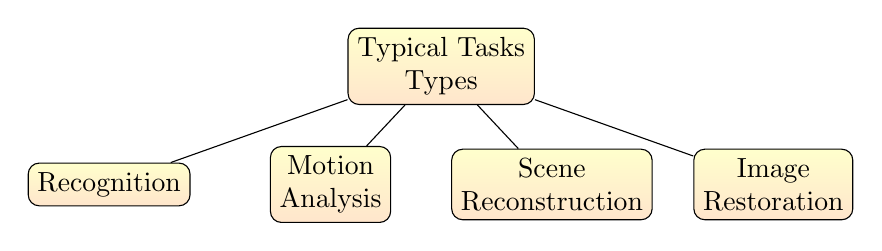
\begin{tikzpicture}[sibling distance=8em,
every node/.style = {shape=rectangle, rounded corners, draw, align=center,
	top color=yellow!20, bottom color=orange!20}]
\node {Typical Tasks\\ Types}
child { node {Recognition}}
child { node {Motion \\ Analysis}}
child { node {Scene \\ Reconstruction}}
child {node{Image \\ Restoration}};
\end{tikzpicture}

\end{frame}


\usebackgroundtemplate{%declare it
\tikz[overlay,remember picture] \node[opacity=0.5, at=(current page.center)] {\includegraphics[height=\paperheight,width=\paperwidth]{Typwall.jpeg}};}

\begin{frame}{TYPICAL TASKS}
\begin{columns}
\column{0.5\textwidth}
\textbf{Other application areas include: \\ Support of visual effects creation for cinema and broadcast, e.g., camera tracking (matchmoving),Surveillance,Tracking and counting organisms in the biological sciences typical tasks.\ Each of the application areas described above employ a range of computer vision tasks; more or less well-defined measurement problems or processing problems, which can be solved using a variety of methods.}
\column{0.6\textwidth}
\centering
\smartdiagramset{
	bubble center node size =3cm,
	distance text center bubble =0.25cm,
	bubble center node color = blue!40,
	bubble center node font = \large,
	bubble node font = \normalfont,
	distance center/other bubbles =0.6cm,
	set color list={orange!80, green!80,magenta!80,
		yellow!80}}
\smartdiagramanimated[bubble diagram]{Typical\\ Tasks,
	Recognition,Motion\\ analysis,Scene\\ reconstruction,Image\\ restoration}
\end{columns}
\end{frame}

\usebackgroundtemplate{%declare it
\tikz[overlay,remember picture] \node[opacity=0.5, at=(current page.center)] {\includegraphics[height=\paperheight,width=\paperwidth]{Recogwall.jpeg}};}

\begin{frame}{\textbf{\underline{(1).RECOGNITION}}}{Typical Tasks} \pause
\setbeamercolor{block body}{bg=orange!40}
\begin{block}{}\textbf{The classical problem in computer vision, image processing, and machine vision is that of determining whether or not the image data contains some specific object, feature, or activity. Different varieties of the recognition problem are described in the literature.}\pause
\end{block}
\begin{columns}
\column{0.5\textwidth}
\begin{itemize}
\item [$\blacksquare$]\textbf{\underline{RECOGNITION TYPES:-}}\pause

\begin{enumerate}
	\item \textbf{Object Recognition.}\pause
	\item \textbf{Identification.}\pause
	\item \textbf{Detection.}\pause
\end{enumerate}
\end{itemize}
\column{0.7\textwidth}
\begin{itemize}
\item [$\ast$]\textbf{\textcolor{red}{Several specialized tasks , such as:}}\pause
\end{itemize}
\begin{itemize}
\item [$\square$]Content based image retrieval.
\item [$\square$]Pose Estimation.
\item [$\square$]Optical Character Recognition (OCR).
\item [$\square$]2D Code Reading.
\item [$\square$]Facial Recognition.
\item [$\square$]Shape Recognition Technology (SRT).
\end{itemize}
\end{columns}
\end{frame}

\usebackgroundtemplate{% declare it
\tikz[overlay,remember picture] \node[opacity=0.4, at=(current page.center)] {\includegraphics[height=\paperheight,width=\paperwidth]{Typwall.jpeg}};}

\begin{frame}{\textbf{\underline{Object Recognition}}}{Recognition Types}\pause
\setbeamercolor{block body}{bg=orange!20}
\begin{block}{}One or several pre-specified or learned objects or object classes can be recognized, usually together with their 2D positions in the image or 3D poses in the scene.\pause
\end{block}
\begin{columns}
\column{0.5\textwidth}
\begin{figure}
\includegraphics[width=\textwidth,height=4cm]{Objreco1.jpeg}
\caption{\underline{(a) \textit{Objects Recognition}}}\pause
\end{figure}
\column{0.5\textwidth}
\begin{figure}
\includegraphics[width=\textwidth,height=4cm]{Objreco2.jpeg}
\caption{\underline{(b) \textit{Object Recognitions}}}\pause
\end{figure}
\end{columns}
\end{frame}

\usebackgroundtemplate{% declare it
	\tikz[overlay,remember picture] \node[opacity=0.6, at=(current page.center)] {\includegraphics[height=\paperheight,width=\paperwidth]{Wall1.jpg}};}

\begin{frame}{\textbf{\underline{Identification And Detection}}}{Recognition Types}
\pause


\begin{tabular}{cc}
	\begin{minipage}{4cm}
		\includegraphics[height=3cm,width=4cm]{Identify1.jpeg}
		
	\end{minipage}
	\begin{minipage}{6cm}
		\setbeamercolor{coloredboxstuff}{fg=black,bg=pink!20}
		\begin{beamercolorbox}[wd=6cm]{coloredboxstuff}
			%\blindtext
			\underline{\large \textbf{\textit{{Identification}}}} - an individual instance of an object is recognized. Examples include identification of a specific person's face or fingerprint, identification of handwritten digits, or identification of a specific vehicle.\pause
		\end{beamercolorbox}
	\end{minipage}
	
\end{tabular}
\begin{minipage}{7cm}
	\setbeamercolor{coloredboxstuff}{fg=black,bg=yellow!40}
	\begin{beamercolorbox}[wd=7cm]{coloredboxstuff}
		%\blindtext
		\underline{\large \textbf{\textit{Detection}}} - the image data are scanned for a specific condition.
		Detection based on relatively simple and fast computations is sometimes used for finding smaller regions of interesting image data which can be further analyzed by more techniques to produce a correct interpretation.
	\end{beamercolorbox}
\end{minipage}
\begin{minipage}{3cm}
	\includegraphics[height=3.5cm,
	width=4cm]{Detect1.jpeg}
\end{minipage}

\end{frame}

\usebackgroundtemplate{%declare it
\tikz[overlay,remember picture] \node[opacity=0.3, at=(current page.center)] {\includegraphics[height=\paperheight,width=\paperwidth]{MotioAna.jpeg}};}

\begin{frame}{\textbf{\underline{(2).Motion Analysis}}}{Typical Tasks}\pause

\setbeamercolor{block body}{bg=green!30}
\begin{block}{}
\textbf{Several tasks relate to motion estimation where an image sequence is processed to produce an estimate of the velocity either at each points in the image or in the 3D scene, or even of the camera that produces the images.}\pause
\end{block}
\begin{columns}
\column{0.6\textwidth}
\centering
\begin{example}\pause
\begin{enumerate}
\item \textbf{\underline{Egomotion}} - determining the 3D rigid motion of the camera from an image sequence.\pause
\item \textbf{\underline{Tracking}} - following the movements of a smaller set of objects in image sequence.\pause
\item \textbf{\underline{Optical Flow}} -  object's apparent motion.\pause
\end{enumerate}
\end{example}
\column{0.5\textwidth}
\begin{figure}
\centering
\includegraphics[width=0.9\textwidth,height=4cm]{MotioAna.jpeg}
\caption{\underline{\textit{Motion Analysis}}}
\end{figure}
\end{columns}
\end{frame}

\usebackgroundtemplate{% declare it
\tikz[overlay,remember picture] \node[opacity=0.2, at=(current page.center)] {\includegraphics[height=\paperheight,width=\paperwidth]{Screen.png}};}

\begin{frame}{\textbf{\underline{(3).Scene Reconstruction}}}{Typical Tasks}\pause
\begin{wrapfigure}{l}{0.5\textwidth}
\centering
\visible<3>{{\includegraphics[width=0.9\linewidth]{Scrnrecon.jpeg}}
\caption{\underline{\textit{Scene Reconstruction}}}}
\end{wrapfigure}
Given one or (typically) more images of a scene, or a video, scene reconstruction aims at computing a 3D model of the scene. In the simplest case the model can be a set of 3D points. More sophisticated methods produce a complete 3D surface model. The advent of 3D imaging not requiring motion or scanning, and related processing algorithms is enabling rapid advances in this field. Grid-based 3D sensing can be used to acquire 3D images from multiple angles. Algorithms are now available to stitch multiple 3D images together into point clouds and 3D models.
\end{frame}

\usebackgroundtemplate{% declare it
\tikz[overlay,remember picture] \node[opacity=0.4, at=(current page.center)] {\includegraphics[height=\paperheight,width=\paperwidth]{restoration.jpg}};}

\begin{frame}{\textbf{\underline{(4).Image Restoration}}}{Typical Tasks}\pause
The aim of image restoration is the removal of noise (sensor noise, motion blur, etc.) from images. The simplest possible noise removal is various types of filters such as low-pass filters or median filters.\pause
\begin{figure}
\centering
\subfloat[Image Restoration\label{fig:a}]{\includegraphics[height=3cm,width=4cm]{restoration.jpg}}\qquad \pause
\subfloat[Method of Restoration\label{fig:b}]{\includegraphics[height=3cm,width=4cm]{Restoration2.jpeg}}
\caption{Figure (A) and (B) showing Image Restoration}
\label{fig:1}
\end{figure}
\end{frame}

\begin{frame}{SCOPE OF COMPUTER VISION}

\begin{columns}[T]
	\begin{column}[T]{5cm}
		\includegraphics[height=3cm]{research-home-areas-computer-vision-407-ud@2X.jpg}
	\end{column}
	\begin{column}[T]{5cm}
		\includegraphics[height=3cm]{download.jpg}
	\end{column}
\end{columns}
\end{frame}
}
\begin{frame}{FUTURE OF COMPUTER VISION}
\textrm{1.}\textbf{The rapid growth of technology has revolutionized computer vision and robotic perception in many frontiers.}\\
\textrm{2.}\textbf{Recent advancements in robotic vision, machine learning, and low-power electronics have allowed researchers and developers to build robotic and automation systems with extraordinary capabilities.}\\
\textrm{3.}\textbf{Although these systems are used in various applications such as self-driving cars, aerial surveying, and human-robot interaction.} \\
\textrm{4.}\textbf{In this brief technical talk, several recent concepts related to robotics and computer vision are presented.}
\textrm{5.}\textbf{Developments have significant economic and scientific impacts on our society and will open new horizons towards the real-time and reliable utilization of computer vision and machine learning systems. }
\end{frame}

\begin{frame}{FUTURE OPPORTUNITIES FOR VISION INDUSTRIES}
\begin{itemize}
\item Depth sensing (near feild)
\item Visual odometry
\item Digital image stabilisation
\item Hyperspectral
\item UV
\item LiDAR
\item Chemical sensors and spectrometers
\item Microphones
\item RFID readers
\end{itemize}

\end{frame}

\begin{frame}{CAREER IN COMPUTER VISION:-}
\begin{columns}[T]
\begin{column}[T]{5cm} 
\textbf{It is one of the most in-demand job titles, perched at the Number 3 spot of Indeed 2018 list of Best Jobs in US. With the rapid flow of investments in AI technologies — both at the startup level as well as within some of the world’s leading technology companies — techies and engineers can restart their career with computer vision.}
\end{column}
\begin{column}[T]{5cm}
\includegraphics[height=3cm]{deeplearning.jpg}
\end{column}
\end{columns}
\end{frame}

\begin{frame}{CAREER IN COMPUTER VISION:-}
\textbf{some of the reasons behind the exponential growth of computer vision}
\begin{itemize}
\item Hardware advancements in terms of availability of GPUs
\item Emergence of deep learning, which has changed our way of performing tasks such as image classification
\item The availability of large datasets such as ImageNet and Caltech 101 that enables beginners and advanced practitioners to work on computer vision applications.
\end{itemize}

\end{frame}

\begin{frame}{CAREER IN COMPUTER VISION:-}

\textbf{How One Can Start Career In Computer Vision:-}

\begin{columns}[t]
\begin{column}{5cm}
Whether you are a beginner or at an intermediate level, the best place to gain practical knowledge about algorithms and computer vision application programming is with \textbf{OpenCV} — an open source computer vision and machine learning software library.
\end{column}
\begin{column}[t]{5cm}
\includegraphics[height=5cm]{OpenCV.jpg}
\end{column}
\end{columns}
\end{frame}

\begin{frame}{MORE ABOUT COMPUTER VISION:-}
\begin{itemize}
\item A commonly used resource in computer vision is Open Source Computer Vision Library (or OpenCV library). 
\item One of the best courses out there to learn more about OpenCV and how it interacts with other computer vision tools is on Udemy. 
\item It has C++, Python and Java interfaces and supports Windows, Linux, Mac OS, iOS and Android. 
\item OpenCV was designed for computational efficiency and with a strong focus on real-time applications. Written in optimized C/C++, the library can take advantage of multi-core processing. 
\item Enabled with OpenCL, it can take advantage of the hardware acceleration of the underlying heterogeneous compute platform.
\item OpenCV has more than 47 thousand people of user community and estimated number of downloads exceeding 14 million.
\end{itemize}

\end{frame}

{
	\usebackgroundtemplate{%
		\tikz\node[opacity=0.7] {\includegraphics[height=\paperheight,width=\paperwidth]{bluee}};}
	\begin{frame}{end}
	\frametitle{References}
	\begin{itemize}
		\item Dana H. Ballard; Christopher M. Brown (1982). Computer Vision.
		\item Huang, T. (1996). Vandoni, Carlo, E, ed. Computer Vision : Evolution And Promise .
		\item Milan Sonka; Vaclav Hlavac; Roger Boyle (2008). Image Processing, Analysis, and Machine Vision.
		\item  Reinhard Klette (2014). Concise Computer Vision.
		\item  Linda G. Shapiro; George C. Stockman (2001). Computer Vision.
	\end{itemize}
\end{frame}

{
	\usebackgroundtemplate{%
		\tikz\node[opacity=1] {\includegraphics[height=\paperheight,width=\paperwidth]{bulb}};}
	\begin{frame}{The End}
	\textbf{
		\Huge{\centerline{Thank You }}}
\end{frame}
}
\end{document} 